 \documentclass[a4paper,12pt]{ctexbook}
\usepackage[margin=2cm]{geometry}
\usepackage{graphicx}
\usepackage{subfigure}
\usepackage{float}
\usepackage[colorlinks,linkcolor=black]{hyperref}%colorlinks启用链接颜色,linkcolor指定对应的颜色
\pagestyle{empty}
\begin{document}

\begin{center}
\huge \textbf{BitBucket简单教程}
\end{center}

\tableofcontents

\newpage

\chapter{git介绍}
Git是一款免费、开源的分布式版本控制系统,用于敏捷高效地处理任何或小或大的项目。

Git 是 Linus Torvalds 为了帮助管理 Linux 内核开发而开发的一个开放源码的版本控制软件。Torvalds 开始着手开发 Git 是为了作为一种过渡方案来替代 BitKeeper,后者之前一直是 Linux 内核开发人员在全球使用的主要源代码工具。开放源码社区中的有些人觉得BitKeeper 的许可证并不适合开放源码社区的工作,因此 Torvalds 决定着手研究许可证更为灵活的版本控制系统。尽管最初 Git 的开发是为了辅助 Linux 内核开发的过程,但是我们已经发现在很多其他自由软件项目中也使用了 Git。例如 很多 Freedesktop 的项目迁移到了 Git 上。
在国内还有阿里云之类的代码托管平台。

\textcolor[rgb]{0.00,1.00,0.25}{本文以BitBucket为例介绍git的使用方法}
\chapter{git平台介绍}
\section{BitBucket简介}
BitBucket是一家源代码托管网站,默认的免费账号,可以总共有5个帐户对你的私有库进行读写。他们给非营利组织(NPO)和大学生免费申请无限账号的机会。何为无限账号:Bitbucket提供每个用户无限公开和私有库,唯一限制的是对私有库有读写权限的帐户总数。适合小型的团体协作。\\
官网地址:\url{https://bitbucket.org/}
\section{GitHub简介}
GitHub 是一个面向开源及私有软件项目的托管平台,因为只支持 Git 作为唯一的版本库格式进行托管,故名 GitHub。GitHub 于 2008 年 4 月 10 日正式上线,除了 Git 代码仓库托管及基本的 Web 管理界面以外,还提供了订阅、讨论组、文本渲染、在线文件编辑器、协作图谱(报表)、代码片段分享(Gist)等功能。目前,其注册用户已经超过350万,托管版本数量也是非常之多,其中不乏知名开源项目 Ruby on Rails、jQuery、python 等。
官网地址:\url{https://github.com}
\section{阿里云简介}
\url{https://code.aliyun.com/}

\newpage
\chapter{创建仓库}
\begin{itemize}
  \item 在\url{https://bitbucket.org}上面创建一个账号。
  \item 进入账号之后,点击创建仓库:
        \begin{figure}[H]
        \centering
        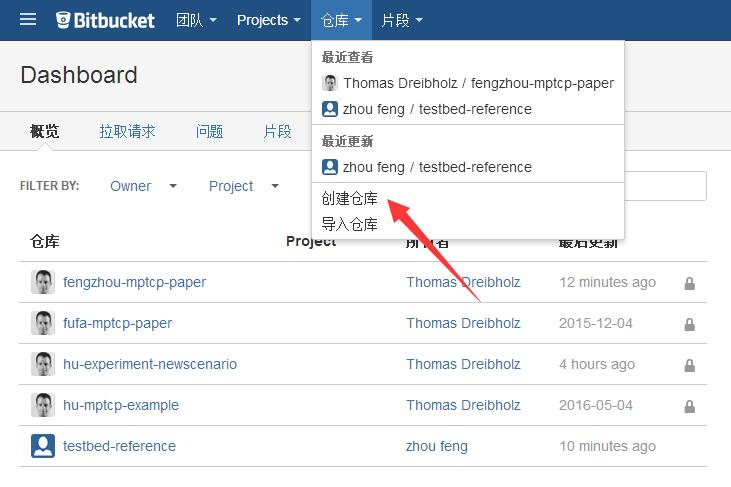
\includegraphics[width=15cm]{figures/create_reponsity.jpg}
        \end{figure}

  \item 创建仓库之后,选择仓库类型:
        \begin{figure}[H]
        \centering
        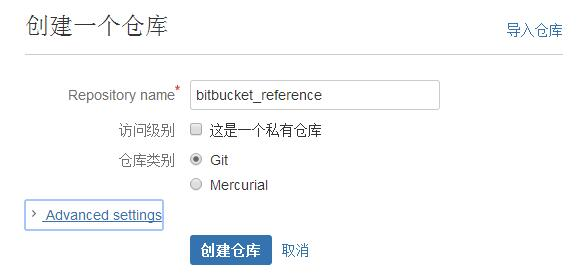
\includegraphics[width=10cm]{figures/create_reponsity_2.jpg}
        \end{figure}

  \item 之后可以参考命令行的相关提示:
        \begin{figure}[H]
        \centering
        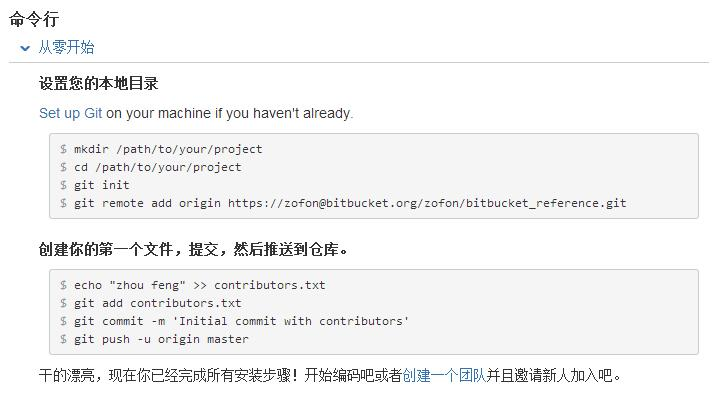
\includegraphics[width=15cm]{figures/create_reponsity_3.jpg}
        \end{figure}
\end{itemize}

\section{上传私钥}
上传公钥之后就可以用公钥登陆bitbucket,不需要输入密码。点击右上角的个人图标,进入个人设置:
\begin{figure}[H]
  \centering
  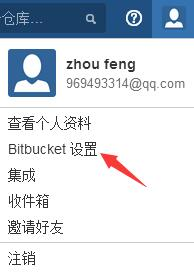
\includegraphics{figures/ssh_set_1.jpg}\\
\end{figure}
然后常规$\rightarrow$安全$\rightarrow$SSH密钥$\rightarrow$添加密钥,按照说明基本没问题。\\
\begin{verbatim}
如下的命令可以将密钥复制到剪切板,比较方便。
安装xclip:sudo apt install xclip
复制到剪切板:cat ~/.ssh/id_rarsa.pub | xclip -sel clip
\end{verbatim}

\newpage
\chapter{团队协作}
\section{邀请别人对你的仓库进行读写}

\section{接受别人的邀请}
别人邀请你加入他的仓库,你会收到一封邮件,按照提示进行操作,完成之后进入自己的Bitbucket账号,点击如下按钮:
\begin{figure}[H]
  \centering
  
\includegraphics[width=10cm]{figures/Bitbucket_button.jpg}
\end{figure}
然后你就会看到当前你的账号下所有的仓库,点击相关的仓库进入。在右上角可以看到克隆地址。

有两种方法可以克隆仓库到本地,HTTP和SSH。

第一种:HTTP是一种比较基础的方法,不需要上传私钥,找到对应的克隆地址,如下:
\begin{figure}[H]
  \centering
  
\includegraphics[width=10cm]{figures/HTTP_clone.jpg}
\end{figure}
在本地终端输入如下命令:
\begin{verbatim}
git clone https://zofon@bitbucket.org/zofon/bitbucket_reference.git
\end{verbatim}

第二种:SSH需要上传私钥,但是比较方便,找到对应的克隆地址,如下:
\begin{figure}[H]
  \centering
  
\includegraphics[width=10cm]{figures/SSH_clone.jpg}
\end{figure}
在本地终端输入如下命令:
\begin{verbatim}
git clone git@bitbucket.org:zofon/bitbucket_reference.git
\end{verbatim}


%=======
%\section{克隆仓库}
%在仓库中找到克隆地址,在bitbucket的仓库里面有两个地址,一个是https克隆地址,另一个是ssh克隆地址。
%它们的用法如下,分别对应两种类型的地址:
%\begin{verbatim}
%git clone https://zofon@bitbucket.org/zofon/design_ubuntu.git
%git clone git@bitbucket.org:zofon/design_ubuntu.git
%\end{verbatim}

\newpage
\section{pull操作基本步骤}
要养成进入仓库先 git pull一下的习惯。这样子可以省去很多麻烦。在一个人使用仓库的时候,只有一个分支,只需要简单的 git pull 命令即可。当多个人在仓库工作的时候,可以用 git pull --all 命令将全部的分支都pull下来,然后处理。

\newpage
\section{push操作基本步骤}
在初始化仓库的时候是需要一个
\begin{itemize}
   \item git add test.tex
   \item git commit -m "Describation"
   \item git push
\end{itemize}
如果权限不是最高权限,不能push到master分支上的时候,可以自己在本地新建一个分支,然后将该分支push到仓库。
\begin{itemize}
  \item git branch zhoufeng
  \item git checkout zhoufeng
  \item git add --all
  \item git commit -m "Descriptions"
  \item git push origin zhoufeng
\end{itemize}

\section{多分支操作}
\begin{description}
  \item[git branch -a]  查看所有的分支。
  \item[git checkout chengxi]   切换到chengxi的分支上。
  \item[git checkout master]    切换回主分支。
  \item[git merge chengxi]  将chengxi分支合并到当前的分支
  \item[git branch -d chengxi]  这个分支合并完了之后可以删掉了。
  \item[git branch -a]  查看所有的分支。
\end{description}

\section{解决冲突}
解决冲突有两种方法:一、merge以前的一个版本,即将之前的版本挪到现在的版本。二、使用git rebase丢弃特定版本之后的数据。相对而言第一种方法处理较好。

\section{回退到某个版本}
如果不小心操作出错了,回退到上一个版本或者上几个版本,用如下命令:
\begin{verbatim}
git reset是指将当前head的内容重置,不会留log信息。

git reset HEAD filename
#从暂存区中移除文件

git reset --hard HEAD~3
#会将最新的3次提交全部重置,就像没有提交过一样。

git reset --hard commit (38679ed709fd0a3767b79b93d0fba5bb8dd235f8)
#回退到 38679ed709fd0a3767b79b93d0fba5bb8dd235f8 版本

根据--soft --mixed --hard,会对working tree和index和HEAD进行重置:

git reset --mixed
#此为默认方式,不带任何参数的git reset,即时这种方式,它回退到某个版本,只保留源码,回退commit和index信息

git reset --soft
#回退到某个版本,只回退了commit的信息,不会恢复到index file一级。如果还要提交,直接commit即可

git reset --hard
#彻底回退到某个版本,本地的源码也会变为上一个版本的内容
例如:我要彻底返回在上一次提交以前的版本。git reset --hrad HEAD~1

git reset --hard
#我要回到上一次提交的版本。
\end{verbatim}
回退到之前的版本之后,可能会出现无法push的情况,这个时候如果是自己一个在使用的话,可以强制push,命令如下:\verb|git push -f|

\newpage
\section{常用命令介绍}
\begin{description}
  \item[git clone] 在如下的位置找到克隆的地址,可以使用该命令将云端的仓库克隆到本地。
        \begin{figure}[H]
        \centering
        
\includegraphics[width=10cm]{figures/clone_address.jpg}
        \end{figure}
        命令如下:git clone https://zofon@bitbucket.org/dreibh/hu-experiment-newscenario.git

  \item[git reflog] 查看提交的版本信息,比较关键的命令。
  \item[git status] 查看当前的提交状态,一般提交之后可以使用这个命令查看。

  \item[git add a.tex] 将改动的文件添加到提交,命令如下:git add *tex ,即自己确定要上传某个文件。
  \item[git add .] 添加当前文件夹的内容到提交,相对--all而言,这个不是递归的。
  \item[git add --all] 递归提交,将文件的所有变动都添加到提交。用于改动文件较多的情况。

  \item[git rm] 删除云端的指定文件,在这之后也是需要commit一下的。

  \item[git commit -am "描述"] 提交命令,-m的意思就是添加描述,-a的意思就是全部提交,比如说之前有添加了没有提交的。
  \item[git commit -m  "描述"] 提交命令,-m的意思就是添加描述,提交这次添加的内容。

  \item[git push -u origin master] 这个在第一次提交的时候使用,第一次需要指定提交的分支。
  \item[git push] 将提交的内容push到云端。
\end{description}

\newpage
\chapter{常见问题}
\section{git commit -m 'Initial commit with contributors' 时候出现错误}
错误信息如下:
\begin{verbatim}
*** Please tell me who you are.

Run

  git config --global user.email "you@example.com"
  git config --global user.name "Your Name"

to set your account's default identity.
Omit --global to set the identity only in this repository.

fatal: unable to auto-detect email address (got 'Administrator@Sc-201608242018.(none)')
\end{verbatim}
这个问题是因为你没有设置相关的用户账号的名字。设置一下即可:
\begin{verbatim}
git config --global user.email "969493314@qq.com"
git config --global user.name "zofon"
\end{verbatim}

\section{git push -u origin master 时候出现错误}
错误信息如下:
\begin{verbatim}
The authenticity of host 'bitbucket.org (104.192.143.1)' can't be established.
RSA key fingerprint is SHA256:zzXQOXSRBEiUtuE8AikJYKwbHaxvSc0ojez9YXaGp1A.
Are you sure you want to continue connecting (yes/no)? yes
Warning: Permanently added 'bitbucket.org,104.192.143.1' (RSA) to the list of known hosts.
Permission denied (publickey).
fatal: Could not read from remote repository.

Please make sure you have the correct access rights
and the repository exists.
\end{verbatim}
这个问题是因为没有添加公钥到Bitbucket上面。添加一个密钥即可。其实这里我也不知道为什么。。。只是这样子可以解决这个问题。

\section{git clone 某个仓库时候出现错误}
错误信息如下:
\begin{verbatim}
remote: Counting objects: 4592517, done.
remote: Compressing objects: 100% (1140430/1140430), done.
error: RPC failed; result=56, HTTP code = 2008.82 MiB | 4.72 MiB/s
fatal: The remote end hung up unexpectedly
fatal: early EOF
fatal: index-pack failed
\end{verbatim}
这个问题是因为克隆的仓库的大小超过了Git的传输字节限制,修改其值即可(这里的单位是Byte):\\
\begin{verbatim}
git config --global http.postBuffer  524288000
\end{verbatim}
524288000就是512MiB\\
所以说要注意自己的仓库的大小。事实上,仓库是不需要多大的。

\section{git pull的时候产生错误}
错误信息如下:
\begin{verbatim}
$ git pull
remote: Counting objects: 27, done.
remote: Compressing objects: 100% (27/27), done.
Connection to bitbucket.org closed by remote host.
fatal: The remote end hung up unexpectedly
fatal: early EOF
fatal: unpack-objects failed
\end{verbatim}
这个问题我也不清楚是什么情况,解决方法就是彻底删掉这个版本库,然后重新克隆。有效。
\end{document}


